\documentclass[%
reprint,
superscriptaddress,
%groupedaddress,
%unsortedaddress,
%runinaddress,
%frontmatterverbose,
%preprint,
showpacs,preprintnumbers,
%nofootinbib,
%nobibnotes,
%bibnotes,
 amsmath,amssymb,
 aps,
%pra,
%prb,
prd,
%prl,
%rmp,
%prstab,
%prstper,
%floatfix,
]{revtex4-1}

\usepackage{float}
\usepackage{graphicx}% Include figure files
\usepackage{dcolumn}% Align table columns on decimal point
\usepackage{bm}% bold math
\usepackage{bbold}
\usepackage{braket}
\usepackage{amssymb,amsmath}
\usepackage{hyperref}% add hypertext capabilities
%\usepackage[mathlines]{lineno}% Enable numbering of text and display math
%\linenumbers\relax % Commence numbering lines

%\usepackage[showframe,%Uncomment any one of the following lines to test
%%scale=0.7, marginratio={1:1, 2:3}, ignoreall,% default settings
%%text={7in,10in},centering,
%%margin=1.5in,
%%total={6.5in,8.75in}, top=1.2in, left=0.9in, includefoot,
%%height=10in,a5paper,hmargin={3cm,0.8in},
%]{geometry}



\usepackage{color}
\usepackage{amsfonts}
\usepackage{subfigure}
\usepackage{array}


\newcommand{\Tr}{\ensuremath{\operatorname{Tr}}}
\newcommand{\tr}{\ensuremath{\operatorname{tr}}}
\newcommand{\Omegaqq}{\ensuremath{\Omega_{\bar{q}q}}}
\newcommand{\vev}[1]{\ensuremath{\left\langle #1 \right\rangle}}
\newcommand{\einh}[1]{\ensuremath{\,\text{#1}}}
\newcolumntype{L}{>{\centering\arraybackslash}m{3cm}}



\newcommand{\overbar}[1]{\mkern 1.5mu\overline{\mkern-1.5mu#1\mkern-1.5mu}\mkern 1.5mu}

\definecolor{bjcol}{rgb}{1,.44,0.13}

% color def's

\definecolor{blue}{rgb}{0,0,1}
\newcommand{\colb}[1]{{\color{blue} #1}}
\definecolor{green}{rgb}{0,1,0}
\newcommand{\colg}[1]{{\color{green} #1}}
\definecolor{red}{rgb}{1,0,0}
\newcommand{\colr}[1]{{\color{red} #1}}
\newcommand{\colJ}[1]{{\color{cyan} #1}}
\definecolor{gray}{rgb}{.5,.5,.5}
\newcommand{\drop}[1]{{\sout{ {\color{gray} #1}}}}
\definecolor{darkgreen}{rgb}{.0,.5,.0}
\newcommand{\colL}[1]{{\color{darkgreen} #1}}


\def\Fig#1{Fig.~\ref{#1}} \def\Tab#1{Tab.~\ref{#1}}
\def\Figs#1{Figs.~\ref{#1}} \def\Tab#1{Tab.~\ref{#1}}
\def\Eqs#1{Eqs.~(\ref{#1})}
\def\Eq#1{Eq.~(\ref{#1})}
\def\eq#1{(\ref{#1})}
\def\eqref#1{(\ref{#1})}
\def\fig#1{Fig.~\ref{#1}}
\def\tab#1{Tab.~\ref{#1}}
\def\eqs#1{(\ref{#1})}
\def\Eqs#1{(\ref{#1})}
\def\sec#1{Sec.~\ref{#1}}
\def\app#1{Appendix~\ref{#1}}
\newcommand{\Phibar}{\ensuremath{\bar{\Phi}}}
\newcommand{\LPQM}{\ensuremath{\mathcal{L}_{\textrm{PQM}}}\xspace}

\def\dbar{{\mathchar'26\mkern-12mu d}}
\def\lA0{{\langle A_0 \rangle}}
\def\bA0{{\bar{A}_0}}
\def\lLA{{\langle L[A_0] \rangle}}
\def\lL{{\langle L \rangle}}
\def\lLc{{\langle L^\dagger \rangle}}
\def\lLAc{{\langle L^\dagger[A_0] \rangle}}


\def\dr{{D\!\llap{/}}\,}
\def\Dr{{D\!\llap{/}}\,}
\def\ipv{\vec{p}\llap{/}}
\def\pslash{p\llap{/}}

\def\0#1#2{\frac{#1}{#2}}

\newcommand{\bsig}{\ensuremath{\bar{\sigma}}}
\newcommand{\lsm}{L\ensuremath{\sigma}M\xspace}
\newcommand{\pT}{\ensuremath{T_0}}
\newcommand{\Tl}{\ensuremath{T_\chi}}
\newcommand{\Ts}{\ensuremath{T_\chi^s}}
\newcommand{\Tchi}{\ensuremath{T_\chi}}
\newcommand{\Td}{\ensuremath{T_d}}
\newcommand{\Tc}{\ensuremath{T_c}}
\newcommand{\muc}{\ensuremath{\mu_c}}
\newcommand{\coloronl}{(color online)\xspace}

\newcommand{\mrm}[1]{\mathrm{#1}}
\def\qbar{\bar{q}}
\newcommand{\sx}{\sigma_{x}}
\newcommand{\sy}{\sigma_{y}}

%%%%%%%%%%%%%% for corrections %%%%%%%%%%%
\newcommand{\colsy}[1]{\textcolor{blue}{#1}}
\newcommand{\colrw}[1]{\textcolor{cyan}{#1}}
\newcommand{\colwjf}[1]{\textcolor{red}{#1}}

%
%%%%%%%%%%%%%%%%%%%%%%%%%%%%%%%%%%%%%%%%%%%%%%%%%%%%%%%%%%%%%%%%%%%%%%%%%%%%%

\graphicspath{{./figures/}{./}}

\begin{document}

\preprint{}

\title{High order generalized susceptibilities of the baryon number under the Polyakov-quark-meson model
}

\author{Shi Yin}
\affiliation{School of Physics, Dalian University of Technology, Dalian, 116024,
  P.R. China}


\author{Wei-jie Fu}
\email{wjfu@dlut.edu.cn}
\affiliation{School of Physics, Dalian University of Technology, Dalian, 116024,
  P.R. China}

%\date{\today}% It is always \today, today,
             %  but any date may be explicitly specified

\begin{abstract}
We study the generalized susceptibilities from kurtosis which is known as the $\chi^B_4/\chi^B_2$ to the $\chi^B_8/\chi^B_2$. The results are obtained under the finite temperature and baryon density. We give the comparison of our results with the lattice QCD results under the vanishing $\mu_B$. We get the numerical results under the Polyakov-quark-meson (PQM) model with the functional renormalisation group (FRG) approch.


\end{abstract}
%\pacs{Valid PACS appear here}% PACS, the Physics and Astronomy
\pacs{11.30.Rd, %Chiral symmetries
         11.10.Wx, %Finite-temperature field theory
         05.10.Cc, %Renormalization group methods
         12.38.Mh  %Quark-gluon plasma
     }                             % Classification Scheme.
%\keywords{Suggested keywords}%Use showkeys class option if keyword
                              %display desired
\maketitle
%\tableofcontents
%%%%%%%%%%%%%%%%%%%%%%%%%%%%%%%%%%%%%%%%%%%%%%%%%%%%%%%%%%%
%%%%%%%%%%%%%%%%%%%%%%%%%%%%%%%%%%%%%%%%%%%%%%%%%%%%%%%%%%%
\section{Introduction}
\label{sec:int}
We ...

%%%%%%%%%%%%%%%%%%%%%%%%%%%%%%%%%%%%%%%%%%%%%%%%%%%%%%%%%%%%%
%%%%%%%%%%%%%%%%%%%%%%%%%%%%%%%%%%%%%%%%%%%%%%%%%%%%%%%%%%%%%
\section{low energy effective model under FRG approach}
\label{sec:LEE}
Here we perform our calculation under the Polyakov loop improved quark-meson model. The effective action which is depend on the evolution of the infrared cutoff scale is
\begin{align}
  \Gamma_k[\Phi]=&\int_x \bigg\{Z_{\psi,k}\bar{\psi} \Big [\partial\!\!\!/ -\gamma_0(igA_0+\hat{\mu}) \Big ]\psi+\frac{1}{2}Z_{\phi,k}(\partial_\mu \phi)^2 \nonumber\\[2ex]
  &+h_k\bar{\psi}\big(T^0\sigma+i\gamma_5 T^i\pi^i\big)\psi+U_k(\rho)-c\sigma \bigg\}\,.
\label{eq:action}
\end{align}
In this work we consider the light quark only, e.g. $u$ quark and $d$ quark, so we have $N_f=2$. The value of index $\mu=0,1,2,3$ and $i=1,2,3$. The integral sign stands for the intergral of the temporal and spatial components, e.g. $\int_x=\int^\beta_0 \int d^3x$. The $\beta$ is the temporal length in the finite temperature field theory $\beta=1/T$. The superfield contain all kind of fields $\Phi=(\psi,\bar{\psi},\phi)$. $\psi=(u,d)$ is the fermion field and $\bar{\psi}$ is the corresponding anti-fermion field. The $O(4)$ invariant effective potential $U_k(\rho)$ is related to the meson field $\phi=(\sigma,\pi^i)$ with $\rho=\phi^2/2$. The $c\sigma$ is the chiral symmetry breaking term. The generators of the $SU(N_f)$ flavor space is give by $T^0$ and $T^i$ which obey the rules:$T^0=1/\sqrt{2N_f}\mathbb{1}_{N_f\times N_f}$ and Tr$(T^iT^j)=1/2\delta^{ij}$. $Z_{\psi,k}$ and $Z_{\phi,k}$ are the wave function renormalisations of the quark and meson fields and $h_k$ is the  running Yukawa coupling. $\hat{\mu}$ is the quark chemical potential matrix, and we have $\mu_B=3\mu$. $A_0$ is the gluon background which is involved through the Polyakov loop in our calculation.\par
The effective action is running with a FRG scale $k$ which is a infrared cutoff. The information of the quantum fluctuations are removed. With the $k$ running from ultraviolet point to infrared point, the behaviour of the fluctuations can be obtained. To describ the running of the effective action with the cutoff scale $k$, we derive the flow equation of the effective action with the Wetterich equation
\begin{align}
\partial_t\Gamma_k[\Phi]=\frac{1}{2}\mathrm{Tr}(G_{\phi\phi,k}\partial_t R^\phi_k)-\mathrm{Tr}(G_{\psi\bar{\psi},k}\partial_t R^\psi_k).
\end{align}
The differential equation is related to the renormalisation group time, e.g. $t=ln(k/\Lambda)$, with the ultraviolet (UV) cutoff $\Lambda$ as the initial point of the flow equation. The low energy effective model is well applied with the scale $k\lesssim 1GeV$. With the $k$ coming to $0$ in the process of solving the differential equation we get the physics value of the effective action. Then the propagators in the flow equation can be derived by the two point correlation functions
\begin{align}
G_{\phi\phi/\psi\bar{\psi}}[\Phi]=\frac{1}{\Gamma^{(2)}_k[\Phi]+R_k}\bigg|_{\phi\phi/\psi\bar{\psi}}.
\end{align}
On the l.h.s of the flow equation is the derivation of the effective action. The analytic form of the flow equations should be calculated by the loop diagram on the r.h.s.\par
The core issue of the PQM model is to investigate the thermodynamical of the system which is related to the meson effective potential for the information of the chiral symmetry breaking it carries. If we only consider the flow equation of the effective potential without the flow of the wave function renormalisation and Yukawa coupling we get the result of the local potential approximation (LPA). Here we give the results of beyond LPA that we take all the quantum fluctuations into account, the running of the $Z_{\phi/\psi,k}$ and $h_{k}$ are completly calculated. The meson and quark wave function renormalisations are split into $Z^{\|}_{\phi/\psi}$ and $Z^{\bot}_{\phi/\psi}$ for the breaking of the $O(4)$ symmetry of the heat bath. However, the spatial components play the most significant role of the physical fluctuations, see \cite{Yin:2019ebz}, so it is reasonable to assume $Z^{\|}_{\phi/\psi}=Z^{\bot}_{\phi/\psi}$ in our work to simplify calculation. \par
Now come to the gluon part, we involve the gluon effect by the glue potential which is related to the Polyakov loop with temporal gluonic background $A_0$
\begin{align}
L(\bm x)=\frac{1}{N_c}\langle \Tr{\mathcal{P}(\bm x)} \rangle ,\qquad \bar{L} (\bm x)=\frac{1}{N_c}\langle \Tr{\mathcal{P}^{\dagger}(\bm x)} \rangle\,,\label{}
\end{align}
the Polyakov loop has the form of
\begin{align}
\mathcal{P}(\bm x)=\mathcal{P}\exp\bigg( ig\int_{0}^{\beta}d\tau A_0(\bm x,\tau) \bigg)\,.\label{}
\end{align}
The glue potential which we emploied in the model, see \cite{Lo:2013hla}, is parameterized as the form below
\begin{align}
U_{glue}(L,\bar{L})/T^4=&-\frac{a(T)}{2}\bar{L}L+b(T)\mathrm{ln}M_H(L,\bar{L})\nonumber \\ 
&+\frac{c(T)}{2}(L^3+\bar{L}^3)+d(T)(\bar{L}L)^2.
\end{align}
$M_H(L,\bar{L})$ stands for the Haar measure which is defined as
\begin{align}
M_H(L,\bar{L})=1-6\bar{L}L+4(L^3+\bar{L}^3)-3(\bar{L}L)^2.
\end{align}
Then we give the parametric form of the factors of the $a,b,c,d$. The factor $a,c,d$ have the same form
\begin{align}
m(T)=\frac{m_1+m_2/t_c+m_3/t_c^2}{1+m_4/t_c+m_5/t_c^2},
\end{align}
and the form of $b$ is
\begin{align}
b(T)=b_1 t_c^{-b_4}(1-e^{b_2/t_c^{b_3}}),
\end{align}
the values of the parameters are fixed by the thermodynamics and can be found at \cite{Lo:2013hla}. The temperature $t_c$ is reduced temperature by $t_c=(T-T_c)/T_c$. We rescale the reduced temperature to make the glue potential accord with the Yang-Mills theory by $(t_c)_{YM}\rightarrow \alpha(t_c)_{glue}$, and $(t_c)_{glue}=(T-T^{glue}_c)/T^{glue}_c$. Here we choose $\alpha=0.7$ and $T^{glue}_c=270\,\mathrm{MeV}$ by fitting the kertosis of the baryon number fluctuation with the lattice results.\par
After the preparation above we derive the flow equation of the effective potential
\begin{align}
  \partial_t V_k(\rho)=&\frac{k^4}{4\pi^2} \bigg [\big(N^2_f-1\big) l^{(B,4)}_{0}(\bar{m}^{2}_{\pi,k},\eta_{\phi,k};T)\nonumber\\[2ex]
&+l^{(B,4)}_{0}(\bar{m}^{2}_{\sigma,k},\eta_{\phi,k};T)\nonumber\\[2ex]
&-4N_c N_f l^{(F,4)}_{0}(\bar{m}^{2}_{q,k},\eta_{q,k};T,\mu)\bigg]\,, \label{eq:flowV}
\end{align}
The definitions of the meson mass and constituent light quark mass are given by
\begin{align}
  \bar{m}^{2}_{\pi,k}&=\frac{V'_k(\rho)}{k^2Z_{\phi,k}}\,,\\[2ex]
  \bar{m}^{2}_{\sigma,k}&=\frac{V'_k(\rho)+2\rho V''_k(\rho)}{k^2 Z_{\phi,k}}\,,\\[2ex]
  \bar{m}^{2}_{q,k}&=\frac{h^{2}_{k}\rho}{2k^2Z^{2}_{q,k}}\,.
\end{align}\par
Under the beyond LPA truncation we adopt in our calculation, the flow equations of wave function renormalisations and Yukawa coupling should be involved. The flow equations of the meson and quark wave function renormalisations i.e. the anomalous dimensions as follows
\begin{align}
  \eta_{\phi,k}&=-\frac{\partial_t Z_{\phi,k}}{Z_{\phi,k}}\,,\qquad
  \eta_{\psi,k}=-\frac{\partial_t Z_{\psi,k}}{Z_{\psi,k}}\,.
\end{align}

%%%%%%%%%%%%%%%%%%%%%%%%%%%%%%%%%%%%%%%%%%%%%%%%%%%%%%%%%%%%%
%%%%%%%%%%%%%%%%%%%%%%%%%%%%%%%%%%%%%%%%%%%%%%%%%%%%%%%%%%%%%
\section{thermodynamics and baryon number fluctuation}
\label{sec:BNF}
For the purpose of calculating the thermodynamics of our system we give the definition of the thermodynamical potential density 
\begin{align}
\Omega[T,\mu]=U_{k=0}(\rho)-c\sigma+U_{glue}(L,\bar{L}),
\end{align} 
it can be solved through the equation of motion $\partial_L\Omega=0$.
From the thermodynamical potential density one can obtain the pressure of the system
\begin{align}
p=-\Omega[T,\mu],
\end{align}
then the baryon number fluctuations can also be computed through the pressure. We give the general expression of the baryon number fluctuation
\begin{align}
\chi^B_n=\frac{\partial^n}{\partial(\mu_B/T)^n}\frac{p}{T^4}.
\end{align}
We can also express the generalized susceptibilities by the cumulants of the baryon number distributions
\begin{align}
\chi^B_1=&\frac{1}{VT^3}\braket{N_B},\\
\chi^B_2=&\frac{1}{VT^3}\braket{(\delta N_B)^2},\\
\chi^B_3=&\frac{1}{VT^3}\braket{(\delta N_B)^3},\\
\chi^B_4=&\frac{1}{VT^3}\big(\braket{(\delta N_B)^4}-3\braket{(\delta N_B)^2}^2\big),\\
\chi^B_6=&\frac{1}{VT^3}\big(\braket{(\delta N_B)^6}-15\braket{(\delta N_B)^4}\braket{(\delta N_B)^2}\nonumber\\
&-10\braket{(\delta N_B)^3}^2+30\braket{(\delta N_B)^2}^3\big)\\
\chi^B_8=&\frac{1}{VT^3}\big(\braket{(\delta N_B)^8}-28\braket{(\delta N_B)^6}\braket{(\delta N_B)^2}\nonumber\\
&-56\braket{(\delta N_B)^3}\braket{(\delta N_B)^5}-70\braket{(\delta N_B)^4}^2\nonumber\\
&-640\braket{(\delta N_B)^2}^4\big).
\end{align}
The angle brackets stand for the ensemble average value and $\delta N_B=N_B-\braket{N_B}$. To compare the results with the lattice simulation further with the experiments we consider the kurtosis $\kappa\sigma^2=\chi^B_4/\chi^B_2$, $\chi^B_6/\chi^B_2$ and $\chi^B_8/\chi^B_2$.


%%%%%%%%%%%%%%%%%%%%%%%%%%%%%%%%%%%%%%%%%%%%%%%%%%%%%%%%%%%%%%%%%%%%%%%%%%%%%%
%%%%%%%%%%%%%%%%%%%%%%%%%%%%%%%%%%%%%%%%%%%%%%%%%%%%%%%%%%%%%%%%%%%%%%%%%%%%%%
\section{initial consitions and numarical results}
\label{sec:NR}
%
%%%%%%%%%%%%%%%%%%%%%%%%%%%%%
\begin{figure*}[t]
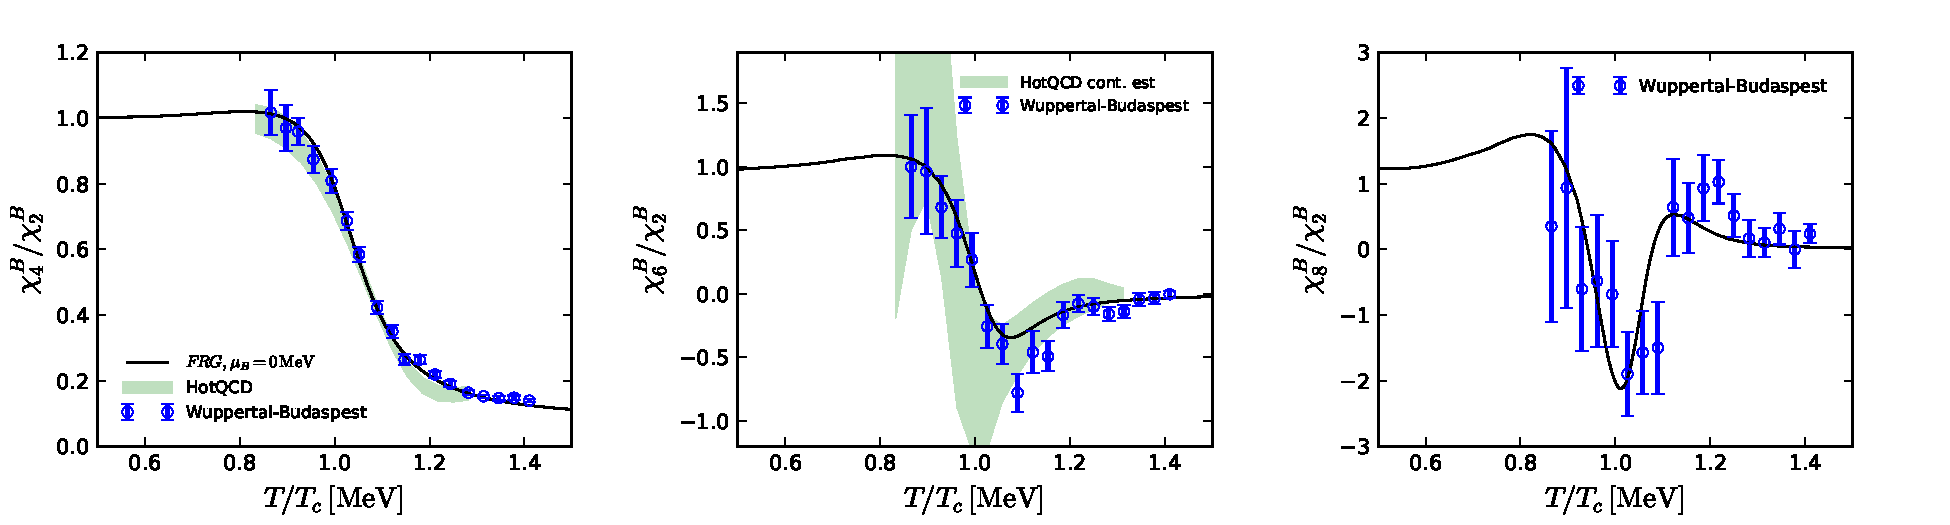
\includegraphics[width=1\textwidth]{mub0}
\caption{This figure give the numerical results of vanishing baryon chemical potential and compare with the results of the lattice simulation. We rescale the lattice data by lattice critical temperature at $\mu_B=0$ which is $T_c=156MeV$. The set rescale parameter of the FRG results $T_c=194MeV$ by fit the FRG kurtosis with the lattice. The HotQCD Collaboration results are from \cite{Bazavov:2017dus,Bazavov:2017tot} the Wuppertal-Budapest Collaboration are from \cite{Borsanyi:2018grb}.}\label{fig:mub0}
\end{figure*}
%%%%%%%%%%%%%%%%%%%%%%%%%%%%%
%
%
 %%%%%%%%%%%
\begin{figure*}[t]
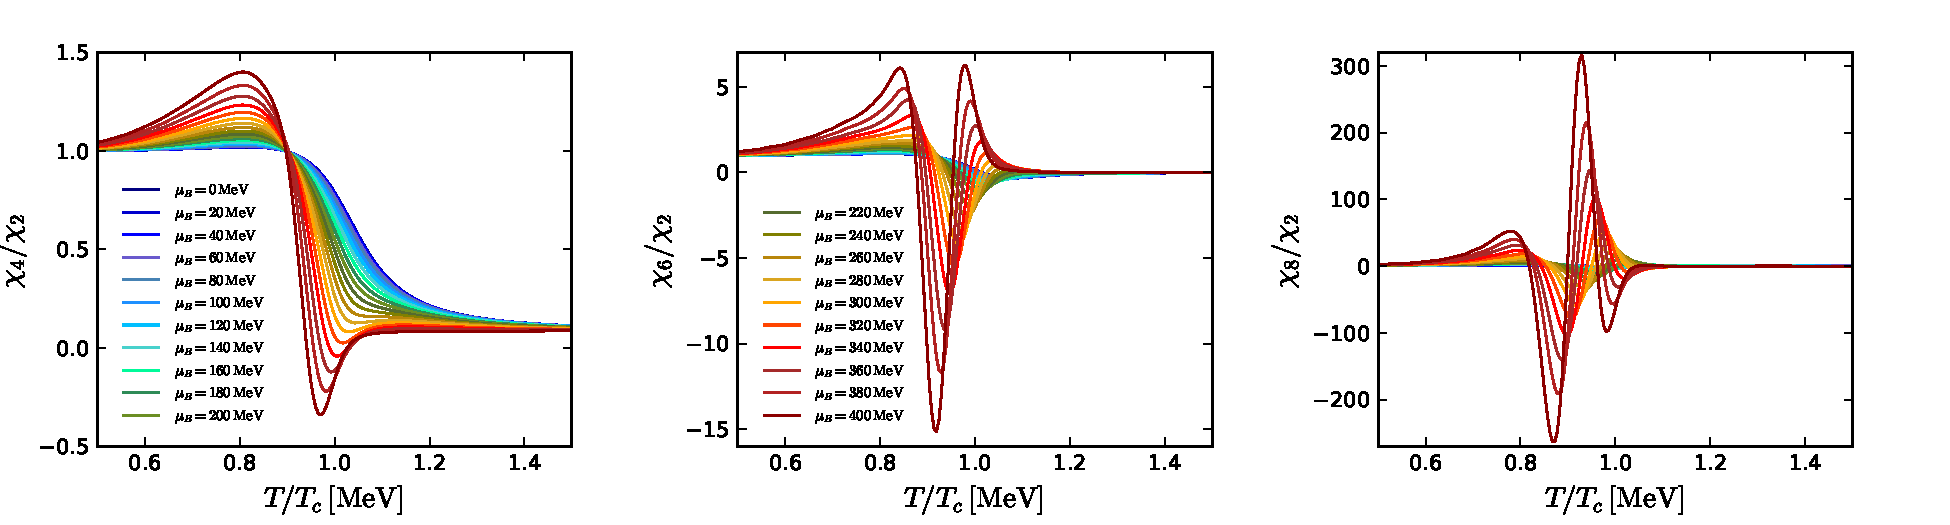
\includegraphics[width=1\textwidth]{finmub}
\caption{The results under baryon chemical potential from $0$ to $400MeV$.}\label{fig:finmu}
\end{figure*}
%%%%%%%%%%
%

For the purpose of solving the flow equation of the effective potential \Eq{eq:flowV} we use the Tylor expansion approach around the expansion point $\kappa$. The renormalised effective potential under the Tylor expansion is
\begin{align}
\bar{U}_k(\bar{\rho})=\sum^{N_u}_{n=0}\frac{\bar{\lambda}_{n,k}}{n!}(\bar{\rho}-\bar{\kappa}_k)^n,\label{eq:Tylor}
\end{align}
with $\bar{U}_k(\bar{\rho})=U_k(\rho)$, $\bar{\lambda}_{n,k}=\lambda_{n,k}/(Z_{\phi,k})^n$, $\bar{\rho}=Z_{\phi,k}\rho$, $\bar{\kappa}_k=Z_{\phi,k}\kappa_k$.
Here we take $N_u=5$ for the well convergence of effective potential. The running cutoff scale dependent expansion point $\kappa_k$ is emploied in our numerical calculation. Then we can get the Tylor expansion flow equation from \Eq{eq:flowV} and \Eq{eq:Tylor} 
\begin{align}
&\partial^n_{\bar{\rho}}\bigg(\partial_t |_\rho\bar{U}_k(\bar{\rho})\bigg)|_{\bar{\rho}=\bar{\kappa}_k}\nonumber\\[2ex]
=&(\partial_t-n\eta_{\phi,k})\bar{\lambda}_{n,k}-(\partial_t\bar{\kappa}_k+\eta_{\phi,k}\bar{\kappa}_k)\bar{\lambda}_{n+1,k}\,.\label{eq:drhodu}
\end{align}
There is another chosen of the expansion point i.e. fixed point which the bare $\kappa$ is independent on the cutoff scale which has a good convergency property of $N_u$, see, e.g.\cite{Pawlowski:2014zaa,Yin:2019ebz}. However, the fixed point expansion may introduce temperature dependence into the Tylor expansion and the thermaldynamics will be influence by this property, so we choose the running point expansion in this work. The running point is the solution of the equation of motion
\begin{align}
\frac{\partial}{\partial \bar{\rho}}\bigg( \bar{U}_k(\bar{\rho})-\bar{c}_k(2\bar{\rho})^{\frac{1}{2}}\bigg)\big|_{\bar{\rho}=\bar{\kappa}_k}=0\,.\label{eq:EoM}
\end{align}
We emphasize that the equation of motion must be satisfied under every value of the infrared cutoff. The renormalised explicit symmetry breaking term is $\bar{c}_k=c/(Z_{\phi,k})^{1/2}$, with the flow $\partial_t \bar{c}_k=(1/2)\eta_{\phi,k}\bar{c}_k$. From \Eq{eq:drhodu} and \Eq{eq:EoM} we can obtain the flow of the renormalised running expansion point
\begin{align}
  \partial_t \bar \kappa_k&=-\frac{\bar c_k^2}{\bar{\lambda}_{1,k}^3+\bar c_k^2\bar{\lambda}_{2,k}}\bigg[\partial_{\bar \rho}\left(\partial_t\big|_{\rho} \bar U_k(\bar \rho)\right)\Big|_{\bar \rho=\bar \kappa_k}\nonumber \\[2ex]
  &+\eta_{\phi,k}^{\perp}\left(\frac{\bar{\lambda}_{1,k}}{2}+\bar\kappa_k\bar{\lambda}_{2,k}\right)\bigg]\,.\label{}
\end{align}
In this work we don't consider the field dependence of the Yukawa coupling and the renormalised Yukawa coupling is $\bar{h}_k=h_k/(Z_{\psi,k}Z^{1/2}_{\phi,k})$.\par
Now we give the ultraviolet of the flow equations i.e. the initial conditions of the differential equations. The ultraviolet cutoff scale is set to $\Lambda=700\,\mathrm{MeV}$. The parameterized effective potential at UV point is
\begin{align}
U_\Lambda(\rho)=\frac{\lambda_\Lambda}{2}\rho^2+\nu_\Lambda\rho\,,
\end{align}
The values of the parameters in the effective potential are $\lambda_\Lambda=11$ and $\nu_\Lambda=(0.830\,\mathrm{GeV})^2$. In addition, the initial values of the explicit chiral symmetry breaking strength and Yukawa coupling are $c=2.82\times 10^{-3}\,\mathrm{GeV}^3$ and $h_\Lambda=10.18$. These parameters are fixed by fitting the vacuum physical observables, i.e., $f_\pi=92\,\mathrm{MeV}$, $m_\psi=300\,\mathrm{MeV}$, $m_\pi=136\,\mathrm{MeV}$,and$m_\sigma=479\,\mathrm{MeV}$.  

%%%%%%%%%%%%%%%%%%%%%%%%%%%%%%%%%%%%%%%%%%%%%%%%%%%%%%%%%%%
%%%%%%%%%%%%%%%%%%%%%%%%%%%%%%%%%%%%%%%%%%%%%%%%%%%%%%%%%%%
\section{summary and outlook}
\label{sec:SO}
%%%%%%%%%%%%%%%%%%%%%%%%%%%%%%%%%%%%%%%%%%%%%%%%%%%%%%%%%%%
%%%%%%%%%%%%%%%%%%%%%%%%%%%%%%%%%%%%%%%%%%%%%%%%%%%%%%%%%%%

\begin{acknowledgments}

The work was supported by the National Natural Science Foundation of China under Contracts Nos. 11775041.

\end{acknowledgments}

%%%%%%%%%%%%%%%%%%%%%%%%%%%%%%%%%%%%%%%%%%%%%%%%%%%%%%%%%%%%%
%%%%%%%%%%%%%%%%%%%%%%%%%%%%%%%%%%%%%%%%%%%%%%%%%%%%%%%%%%%%%

% The \nocite command causes all entries in a bibliography to be
% printed out whether or not they are actually referenced in the
% text. This is appropriate for the sample file to show the different
% styles of references, but authors most likely will not want to use
% it.  \nocite{*}

%\bibliography{refspec}% Produces the bibliography via BibTeX.
\bibliography{ref-lib}% Produces the bibliography via BibTeX.


\end{document}
